 %%LATEX header ********************************************
\documentclass[a4paper, 12pt, titlepage]{article}
\usepackage[utf8]{inputenc}
\usepackage[T1]{fontenc}
\usepackage[danish]{babel}
\usepackage{cite,refstyle,adjustbox,graphicx,amsmath,amssymb,subcaption,varioref,titlesec,comment,amsthm}
\usepackage{mathtools}
%\usepackage{epstopdf}
\usepackage{booktabs}
\usepackage{geometry}
\usepackage{setspace}
\usepackage{pgf,tikz}
\usepackage{fancyvrb}
\usepackage{parskip}
%%************************************************************
%%Teorem miljøer 
\newtheorem{antag}{Antagelse}
\newtheorem{teo}{Teorem}
%%************************************************************
%%Andet setup
\onehalfspacing
%%************************************************************
%% Makro
\newcommand{\indep}{\perp\!\!\!\perp}
\newcommand{\saa}{\Leftrightarrow}
\newcommand{\pd}[2]{\frac{\partial #1}{\partial #2}}
\newcommand{\Lagr}{\mathcal{L}}
%%************************************************************
%% Om forfatteren
%%************************************************************
\author{Simon Harmat og Niels Bækgård}
\title{Øvelse i produktivitetspolitik}
\date{\today}
\begin{document}
%\maketitle
%\tableofcontents
Hermed en analyse og vurdering af produktivitetsudfordringer særligt i Region sjælland

\section{Indledning}
Vi er interesserede i at undersøge, om der kunne være uudtømte effekt ved fra urbanisering i region Hovedstaden set i forhold til region Sjælland. 
\subsection{Motivation}
Der er store forskelle i timeproduktiviteten mellem region Sjælland og region Hovedstaden. En del af disse forskelle skyldes ganske givet branchesammensætning, hvor mere produktive brancher fylder mere i region Hovedstaden end de gør i region Sjælland. Men det kan ikke forklare det hele.

Hvis man i stedet sammenligner samme brancher og dermed ser på, hvad produktivitetsforskellen måtte være her, da vil det være muligt at udrede om der gives urbane produktivitetseffekter. Dette kalder vi for \emph{urban learning}.
\section{Teori}
\subsection{Agglomeration}

Agglomeration og produktivitet
Agglomerationsøkonomi betegner en positivt eskternalitet som opstår, når økonomiske agenter (personer og virksomheder) drager nytte af være fysisk tæt på hinanden. Teorisk kan denne effekt opstå af flere forskellige årsager. D

Fælles brug af ( lave faste omkostninging) 



Matching


Vidensdeling 

Agglomeration kan også øges ved bedre infrastruktur for på den måde at mindske den fysiske afstand mellem byer og mennesker

Skriv lidt om lokaliseringsøkonomi og urbanisering, forskel mellem de to. Vores mål adskiller ikke de to. I meta-analysen skriver de at det ikke gør den store forksel overordnet
\subsection{Produktivitetskommissionen}
\subsection{Debatindlæg fra CE}
\section{Metode}
\subsection{Målning af agglomertaionseffekter med effektiv tæthed }

Der findes flere fremgangsmetode når agglomerationseffetker skal estimeres. Fælles for metoderne er at danne et mål som skal repræsentere skala af økonomiske aktivitet i en geografisk kontekst,indgå som variable i estimationen af produktiviteten og dermed modellere eksternaliteten ved agglomeration. I meta-analysen \cite{melo2009meta} gennemgår forfattterne evolutionen af disse forskellige metoder. De tidligeste eksempler fokuserede udelukkende lokale byeffekt og berorede sig ofte på indbyggerantal. Problemet ved disse mål er, at indbyggerantal i et givent område ikke alene er et udtryk for den stedsbestemte økonomiske aktivitet, men indbyggerantallet vil også være et udtryk for bystørrelser.

Sidenhen blev beskæftigelsestætheden indtroduceret. Fordelen ved dette mål er at den lokale beskæftigelse mere isoleret udtrykker den økonomiske aktivitet, og derved er et bedre mål for produktivitetsfordele. Tæthedsaspektet gør også målet robust overfor størrelsesforskellige områder imellem. 

Fælles for begge mål er, at der implicit i målene er en antagelse om afgrænsede markeder, områder imellem. Dette betyder, at områdernes relative afstand ingen betydning har, og områderne kan ikke drage nytte af hinandensmarkedede, og derved opnå spillover effekter. Spillover effekte i form af større arbejdsmarkeder mht. matching, vidensdeling eller specialisering. For både at tage højde for skalaen af økonomisk aktivitet og nærheden af andre lokaløkonomier eller markeder udviklede nogle studier en anden metode.  

Graham introducere Denne parameter måler hele den økonomiske aktivitet, men tager ikke højde for lokaliserings- og urbaniseringsøkonomi. Selv om dette kan være interessant, så hævder Graham at dette ikke har den store effekt når man ønsker at esitmere eksternaliteten ved agglomerationsfordele. Forskellen på lokaliseringsøkonomi og ur
Graham har estimeret forskellige effekter ved urbanisering vs. clusters i et andet papir (Graham 2006) 

 
 Lokaliseringsøkonomi
• Vidensspillovers baseret på ensartet produktion
– Klynger, ældre industrier – Urbaniseringsøkonomi
• Videsspillovers baseret på diversitet
– Massen af forskellighed, nyere industrier

Til skalaen af økonomiske aktivitet benytter vi antal beskæftigede lønmodtagere efter arbejdssted på kommuneniveau. For at medtage intensiteten på tværs af kommunerne, sætter vi antal beskæftigede i forhold til arealet af kommunerne. Fordelen ved at benytte beskæftigelsestæthed istedet for indbyggertætheden er: 1) antal beskæftigede fanger bedre produktivitetsfordelen ved geografiske konsentreret økonomisk aktivitet, mens at indbygger også vil agere som proxy for urbanisering og eventuelle traffik omkostninger. Ved at benytte tætheden, altså antal eskæftigede lønmodtagere forhold til areal, gør målet robust overfor forskellige kommune størrelser \cite[pp. 335.]{melo2009meta}...

%%%Figur
\begin{figure}[tb]
    \centering
    \begin{subfigure}[b]{0.49\textwidth}
        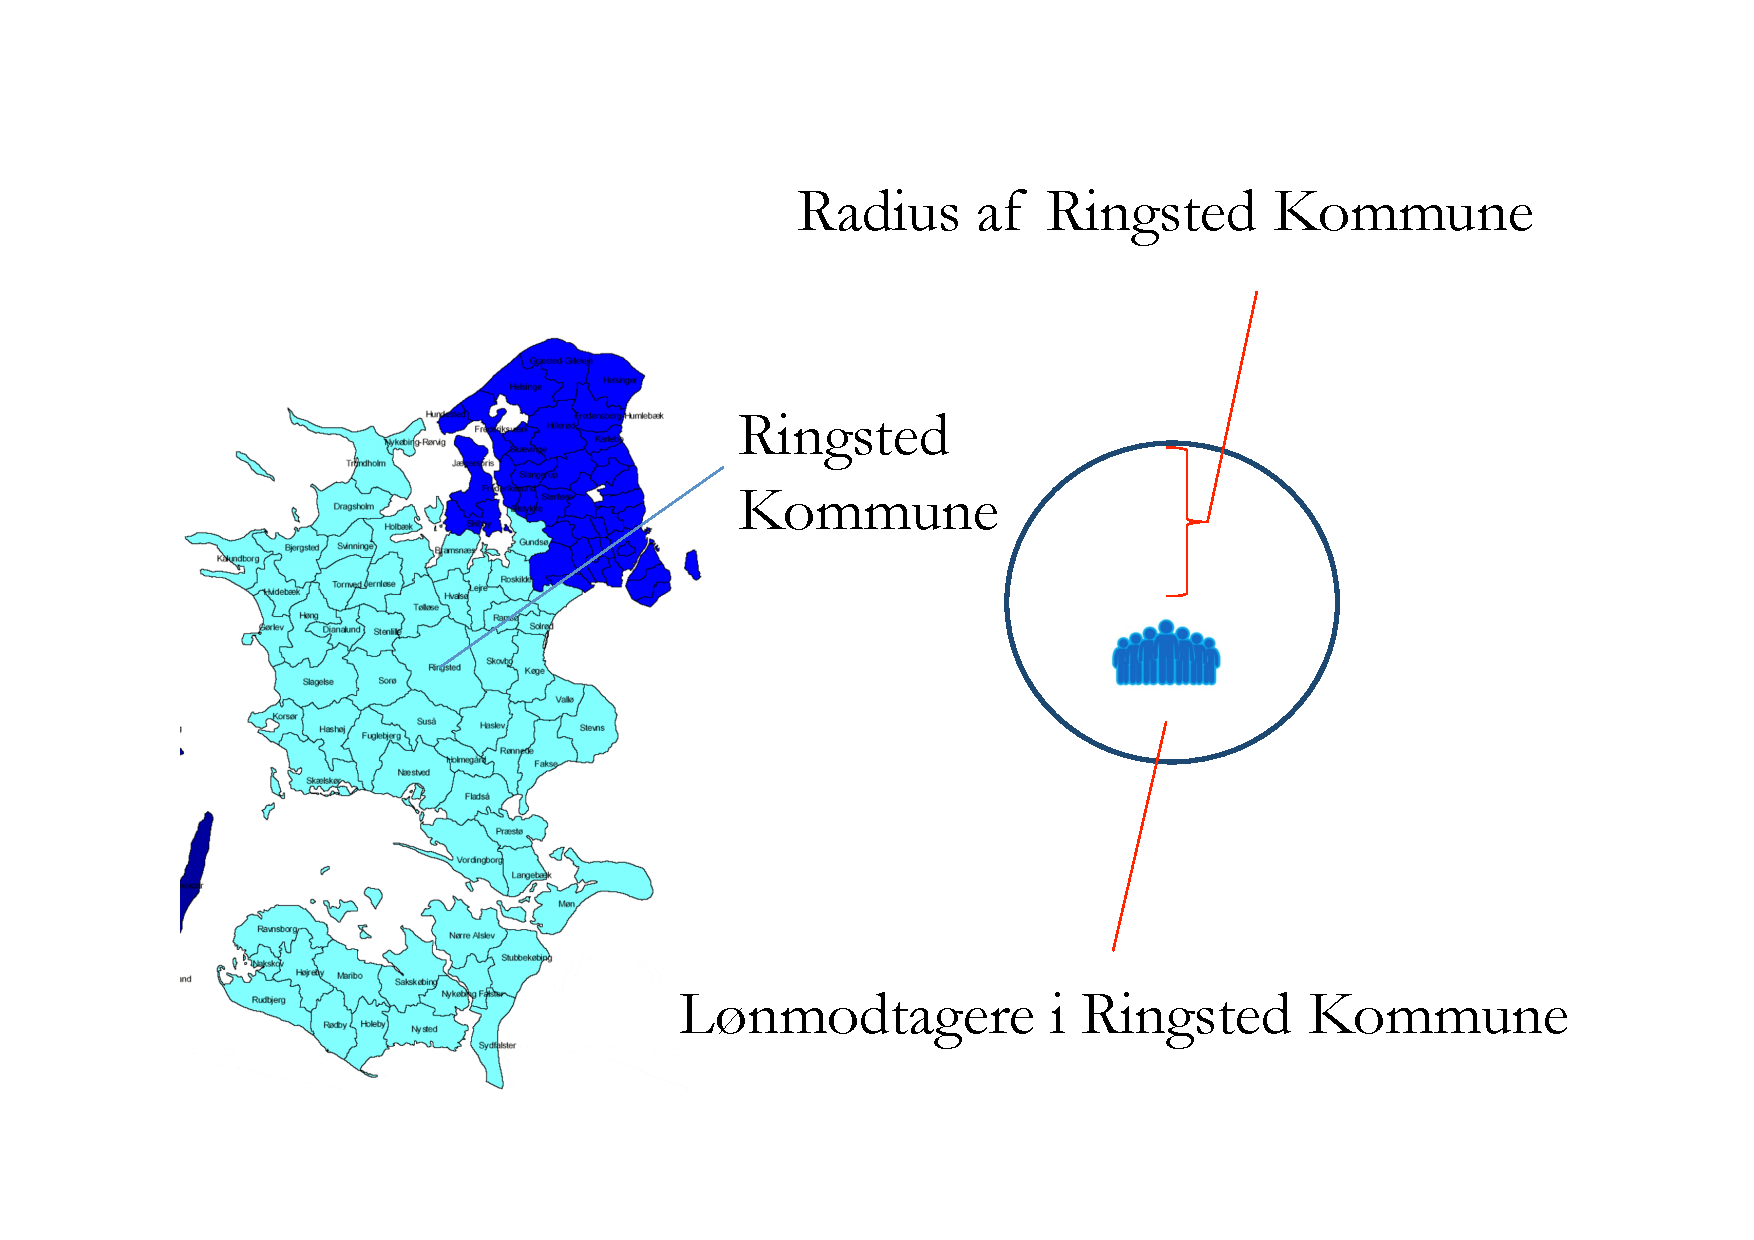
\includegraphics[width=\textwidth]{del1.pdf}
        \caption{Del 1}
        \label{fig:del1}
    \end{subfigure}
    \begin{subfigure}[b]{0.49\textwidth}
        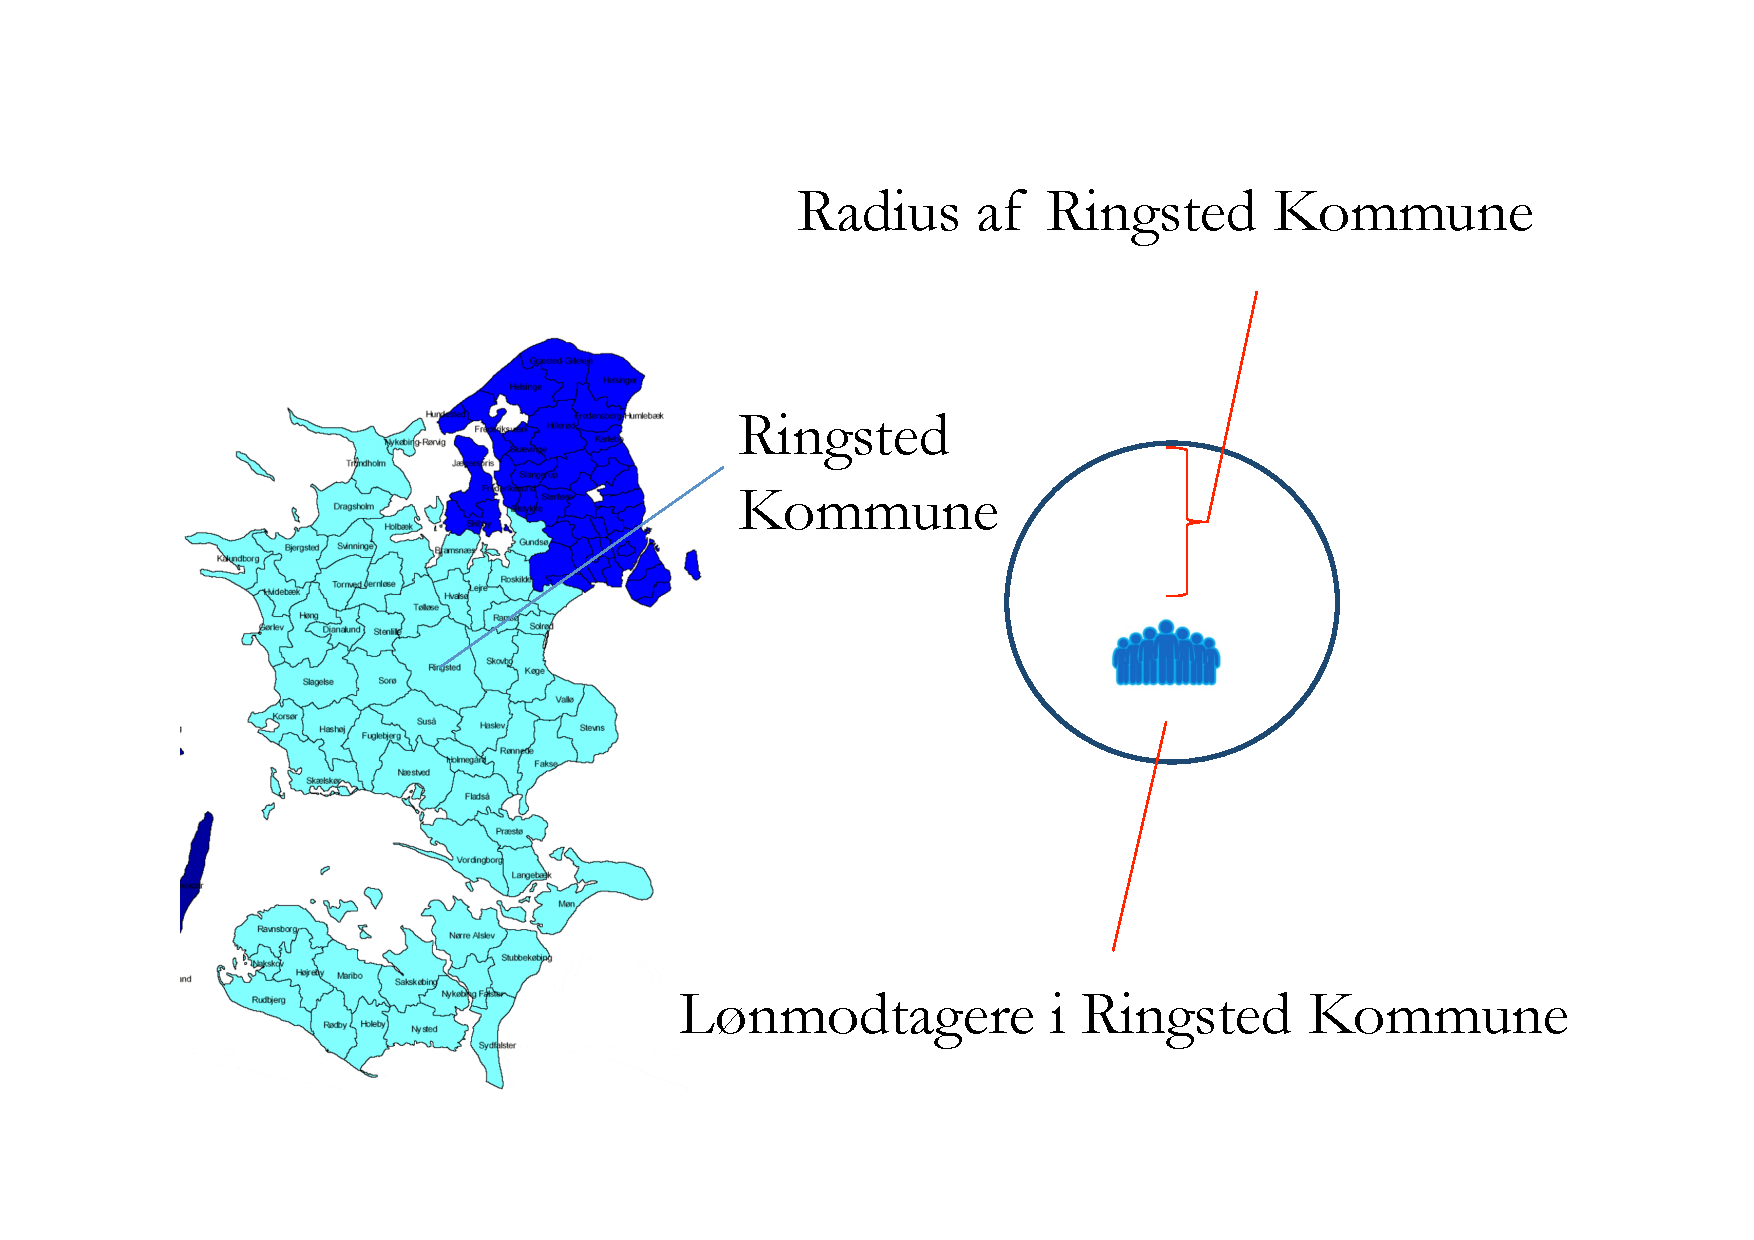
\includegraphics[width=\textwidth]{del1.pdf}
        \caption{Del 2}
        \label{fig:del2}
    \end{subfigure}
	\caption{Caption here}
	\label{fig:SimonsFigur1}
\end{figure}
  

$ED$ er en afstandsparameter, der måler, hvor meget arbejdskraft der der tilgængelig for den enkelte virksomhed, når der tages højde for den geografiske nærhed. Således er det i modellen muligt for en virksomhed i Lolland kommune at rekrutere arbejdskraft i Aalborg, men disse 

\begin{equation}
   ED^j_t = \frac{L^j_t}{Radius_j} + \sum_{k=1}^{k \neq j} \frac{L^k_t}{d_{kj}}, \quad Radius_j = \sqrt{\frac{A_j}{\pi}}
 \end{equation} 
 hvor $d_{kj}$ er afstanden mellem kommune $k$ og $j$. 
 
 
For at finde afstandene mellem alle 98 kommuner i Danmark, benytter vi en såkaldt API. En API gør det muligt at automatisere forspørgelser til en server, i dette tilfælde til servicen Google Maps gennem programmet \textsf{R}. Ved at sende navnet på kommune returnere Google Maps en lokalation i form af koordinat i breddegrader og længdegrader. Vi antager at denne lokation er det approksimative økononomiske midtpunkt af en given kommune. 


Dernæst udregner vi afstandene mellem to kommuners koordinater vha. Haversine-formel\footnote{Skriv en lille historie}. Haversine-formel beregner den korteste afstanden mellem to punkter på en sfære, hvilket netop giver fulgefulgt mellem to kommnuernes midtpunkter. Således kan vi udregne afstandende på kryds og tvær af alle kommuner i en $98\times 98$ symmetrisk matrice. 

\section{Data}
\section{Estimation}
Vi ønsker at estimere følgende output dataset
\begin{equation}
	\ln Y_{it}^{pj} = \alpha^p_0 + \ln K_{it} + \ln L_{it} + ED^j_{t} + \omega^p_{t}
\end{equation}
hvor $i$ er virksomhedsindeks, $p$ kommuneindeks, $t$ angiver tidspunkt i år og $j$ angiver kommune. 
\section{Praktisk case/vinkel}
\section{Konklusion}



\paragraph{Kvalitetsjusteret arbejdskraft}



\paragraph{Levihnson og Petrin}
Hvad nu hvis jeg skriver noge

Syntaksen for at citere er \cite[pp. 211ff.]{melo2009meta}. 

 % paragraph levihnson_og_petring (end)



\bibliography{prodBib.bib}
\bibliographystyle{plain}
\end{document}